\subsection{Testing for Exposed Session Variables - OTG-SESS-004}\label{exposed_session_variables}
\subsubsection{BANK-APP}
\begin{longtable}[l]{ p{2.3cm} | p{.79\linewidth} }\hline
    & \textbf{BANK-APP}
    \hfill CVSS Score: 6.5 \progressbar[filledcolor=BurntOrange]{0.65}
    \\ \hline
    \textbf{Observation} & On the first visit no session variables are set for the session. After the first login there is a cookie called \code{PHPSESSID} with a 26 character value. Even after logging in and out several times, even with another account, the value for \code{PHPSESSID} stays the same. Copying that value and inserting it into another browser with JavaScript while the user is logged in, the other browser also has access to that account, i.e. the session cookie is valid for several sessions for one account at the same time. \\
    \textbf{Discovery} & Using the developer tools of Chrome or Firefox the cookies set can be seen. Furthermore, with ZAP the traffic was scanned for session cookies and session variables. \\
    \textbf{Likelihood} & To read the cookies a hacker only needs to read out the HTTP headers. Executing the JavaScript code \code{document.cookie = "PHPSESSID\allowbreak =SESSION\_COOKIE\_VALUE"} in the browser while on the website sets the cookie. Manually accessing an URL, which usually only a logged in user can see, the hacker is now also logged in. \\
    \textbf{Impact} & Since copying the session cookie grants access to a logged in user there are many risks. \\
    \textbf{Recommen\-dations} & Session cookies should only be valid for the current browser and IP address. \\ \hline
    \textbf{CVSS} &
        \begin{tabular}[t]{@{}l | l}
            Attack Vector           & \textcolor{red}{Network} \\
            Attack Complexity       & \textcolor{red}{Low} \\
            Privileges Required     & \textcolor{red}{None} \\
            User Interaction        & \textcolor{Green}{Required} \\
            Scope                   & \textcolor{Green}{Unchanged} \\
            Confidentiality Impact  & \textcolor{red}{High} \\
            Integrity Impact        & \textcolor{Green}{None} \\
            Availability Impact     & \textcolor{Green}{None}
        \end{tabular}
    \\ \hline
\end{longtable}

\subsubsection{SecureBank}
\begin{longtable}[l]{ p{2.3cm} | p{.79\linewidth} }\hline
    & \textbf{SecureBank} \\ \hline
    \textbf{Observation} & Visiting the website a cookie called \code{Main\_session} is set with a 26 character value. Changing the cookie value and therefore copying it is not possible since it can be only modified via HTTP. If sending HTTP headers with the cookie and its value via \code{curl}, it returns the error message ``You have to be logged in to see this''. \\
    \textbf{Discovery} & Using the developer tools of Chrome or Firefox the cookies set can be seen. Furthermore, with ZAP the traffic was scanned for session cookies and session variables. \\
    \textbf{Likelihood} & N/A \\
    \textbf{Impact} & N/A \\
    \textbf{Recommen\-dations} & N/A \\ \hline
    \textbf{CVSS} & N/A \\ \hline
\end{longtable}

\subsubsection{Comparison}
Both applications use cookies to store the session variable. The vulnerability is given with BANK-APP since copying the session cookie gives a hacker access to the account, if the user is logged in. With SecureBank this is not possible. Figure~\ref{fig:session_cookie} shows the \code{curl} command for trying to gain access to a page only a logged in user can see.

\begin{figure}[ht]
	\centering
	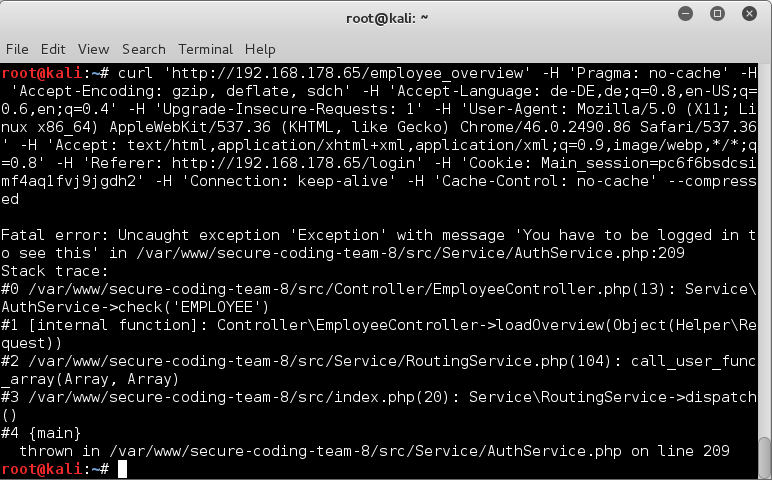
\includegraphics[width=.8\linewidth]{figures/OTG-SESS-004.png}
	\caption{Sending session cookie to SecureBank with \code{curl} command}
	\label{fig:session_cookie}
\end{figure}

\clearpage